\documentclass[letterpaper]{article}
\usepackage[submission]{aaai2027}
\usepackage[hyphens]{url}
\usepackage{graphicx}
\urlstyle{rm}
\def\UrlFont{\rm}
\usepackage{natbib}
\usepackage{caption}
\frenchspacing
\usepackage{amsmath}
\usepackage{booktabs}
\usepackage{enumitem}
\usepackage{microtype}
\usepackage{tabularx}
\usepackage{xcolor}
\usepackage{tikz}
\usepackage{xspace}
\usetikzlibrary{arrows.meta,fit,positioning,shapes.geometric}

\pdfinfo{
/TemplateVersion (2027.1)
}

\newcommand{\system}{\textsc{Agent Nebula}\xspace}
\newcommand{\artifact}[1]{\texttt{#1}}

\title{Supplementary Material for:\\
Are Long-Running Agents Making Progress?\\
A Longitudinal Study of Artifact Progress, Repeated Mutation, and Continuity}
\author{Anonymous Submission}
\affiliations{}

\begin{document}
\maketitle

\begin{abstract}
Long-running agents can modify a workspace for days across many session boundaries.
When they stop, action counts, commits, and final artifacts do not reveal
whether activity accumulated into durable and validated progress or repeatedly
overwrote, abandoned, and rediscovered the same work.  Existing trajectory
studies characterize actions within benchmark attempts, while studies of
long-lived agents focus on task outcomes or internal memory degradation.  We
instead make the persistent workspace the longitudinal unit of analysis.
We introduce a source-linked projection that connects native Claude, Codex, and
Gemini actions to stable artifact identities, lifecycle effects, event time,
and session boundaries without introducing semantic labels or aligning the
timeline to Git commits.  We use it to study six real software and autonomous-
research projects through introduced-artifact persistence, later reuse,
validation association, repeated mutation, workspace-activity migration, and
cross-session continuity.  Under the admitted local projection, across 551
native root sessions and 181,303 Tool actions,
89.3--97.1\% of eligible mutations are later revisited, yet action volume only
weakly orders the cross-project reuse relation ($\rho=0.20$).  Repeat-observed
episodes account for 74.5--90.8\% of mutation episodes, with 42.0--86.7\% of
episodes concentrated in the most-mutated 10\% of identities.  Source coverage
is itself consequential: recognized successful validation appears in all six
cases after projection repair, and named Skills show no supported repeatable
separation in the only eligible comparison.  In 320 stratum-specific public
task/topic selections,
path-local transitions and 2--3-intervening-call module returns recur, but persistent
artifact lineage and cross-session re-grounding remain unobservable.
Finally, a source-direct 120-question conformance experiment found the frozen
implementation answering only 32/60 artifact-linked and cross-session facts
correctly (2026-07-23).  Root-cause repair of session joins, failed-call
effects, shell path extraction, and event workdir handling brings the current
revision to 60/60 on the corrected benchmark---a repair-corpus conformance
result, not a general exact-fact capability claim.
\end{abstract}

\section{Introduction}

An increasingly common workflow gives an agent a broad idea, leaves it to work
inside one repository for two or three days, and inspects the result later.
The returned workspace may contain hundreds of tool calls, dozens of commits,
and substantial code, prose, tests, and experimental output.  This volume
looks productive but does not answer the question the user actually has:
\emph{did the work converge into durable, validated progress?}

Final state and commit history are necessary but lossy views of that question.
They omit reads, failed validations, transient artifacts, overwritten attempts,
and the cost of re-establishing context after a session boundary.  Aggregate
counts retain activity volume but erase which artifacts actions concerned and
whether later work reused or replaced them.  A raw log retains detail, yet its
session-local linear order does not directly expose a workspace lineage that
continues after one context disappears.  Context management can rapidly weaken
earlier plans~\cite{mehta2026plans}, and reliability can change over long chains
of sessions~\cite{zhu2026aging}.

Fine-grained trajectory analysis is not new.  Prior work mines action
sequences and repeated behaviors in software-engineering agents
~\cite{bouzenia2025trajectories}, measures validation and context-gathering
behavior under task and model confounds~\cite{mehtiyev2026behavioral}, and
shows that agents may reach a correct intermediate state and later overwrite
it~\cite{kim2026trajeval}.  ProcGrep represents trajectories as action
procedures and supports deterministic pattern queries and behavioral
fingerprints~\cite{oderinwale2026procgrep}.  Persistent file workspaces and
multi-session tasks are also established system mechanisms and settings
~\cite{zhou2026orspace}.  These results rule out generic claims about first
trajectory analysis, edit loops, validation gaps, fingerprints, or persistent
workspaces.

The remaining gap is longitudinal and artifact centered.  A benchmark attempt
usually ends when one patch is scored; a persistent project continues while
code, papers, datasets, results, and documentation acquire histories of their
own.  We ask how action volume relates to three observable dimensions:
\emph{introduced-artifact persistence}, whether an observably introduced
artifact persists; \emph{reuse}, whether later work returns to it; and
\emph{validation association}, whether an adapter-recognized successful
validation precedes the artifact's next mutation or deletion.  We keep these dimensions
separate instead of combining them with arbitrary weights.  Their conjunction
is useful shorthand for durable, reused, and validation-associated artifact
progress, not a scalar quality score.

We build this study directly on native Agent records.  The existing
\artifact{agent-session} adapters parse Claude, Codex, and Gemini.  A thin
repository projection retains all admitted Tool actions, resolves qualified
file effects, attempts to preserve explicit rename lineage and session
identity, and orders events by Agent action time.  Git contributes final tracked state and
optional content-survival evidence, but commits never define the time axis.
The same facts drive both quantitative analyses and the auxiliary \system
replay; visual layout is not a statistical measurement.  We independently
test the projection rather than treating its output as truth.

This paper makes three contributions:

\begin{enumerate}[leftmargin=*,itemsep=2pt]
  \item a projection-conditioned longitudinal characterization of how Agent activity,
  artifact persistence, reuse, validation, repeated mutation, workspace
  activity, and session
  continuity interact across six real coding and autonomous-research projects;
  \item a deterministic, source-linked measurement protocol for stable
  artifact identity and cross-session lineage, together with a source-direct
  conformance benchmark on which the frozen implementation failed (32/60
  artifact-linked and cross-session facts, 2026-07-23) and the repaired
  revision now answers 60/60, reported as repair-corpus conformance rather
  than a general exact-fact capability claim; and
  \item a reproducible coverage discipline that separates measured results,
  coverage-only evidence, implementation disagreement, and N/A conditions
  instead of treating missing or projected trajectory evidence as observed
  truth.
\end{enumerate}

\section{Problem Setting}
\label{sec:problem}

\subsection{Persistent Work Rather Than Isolated Sessions}

Let a workspace $W$ persist while sessions $S=(s_1,\ldots,s_m)$ execute native
Tool actions $A=(a_1,\ldots,a_n)$.  Each action may read, create, mutate,
rename, or delete zero or more artifacts.  Sessions partition model context;
they do not reset $W$ or terminate an artifact's history.  Our unit of analysis
is one repository lineage over the complete observation interval, with
project-level cases kept separate.

Action time is ordered by native timestamp and stable source identifier.  A
commit can occur between actions and can anchor a final-state query, but it
does not replace the action order.  This distinction is important because an
agent can explore, fail, create temporary files, and revert changes before any
commit.

\subsection{Observable Progress Without Semantic Gold}

We do not infer intent, failure cause, reflection, or waste from file motion.
Instead, we measure source-verifiable process facts:

\begin{itemize}[leftmargin=*,itemsep=2pt]
  \item \textbf{Introduced-artifact persistence}: final existence or tracked
  state for artifacts observably introduced during the trace; existing-file
  writes have unknown content durability without independent evidence;
  \item \textbf{Reuse}: a later source-linked access to the same artifact
  lineage and its event, time, and session distance; and
  \item \textbf{Validation association}: distance from mutation to the next
  adapter-recognized successful test, check, or build action before that
  artifact's next mutation or deletion.
\end{itemize}

Recognized validation proves only that the adapter observed a successful
command, not that it covered a particular mutation; unrecognized commands and
unknown statuses remain coverage gaps.  A file that is never revisited is an observed orphaned
artifact, not automatically useless.  Repeated tests or edits are process
patterns, not automatically waste.  Skill and harness analyses therefore
report temporal association, never causality, in the observational corpus.

Figure~\ref{fig:process-measures} makes the measurement relationships explicit.
The study follows Agent action time through session boundaries, keeps artifact
histories distinct, and measures survival, later reuse, validation distance,
and observable re-grounding.  The figure is a definition schematic rather than
an empirical result; the corresponding result plots are generated from the
six-project source rows in Section~\ref{sec:evaluation}.

\begin{figure*}[t]
\centering
\resizebox{0.96\textwidth}{!}{%
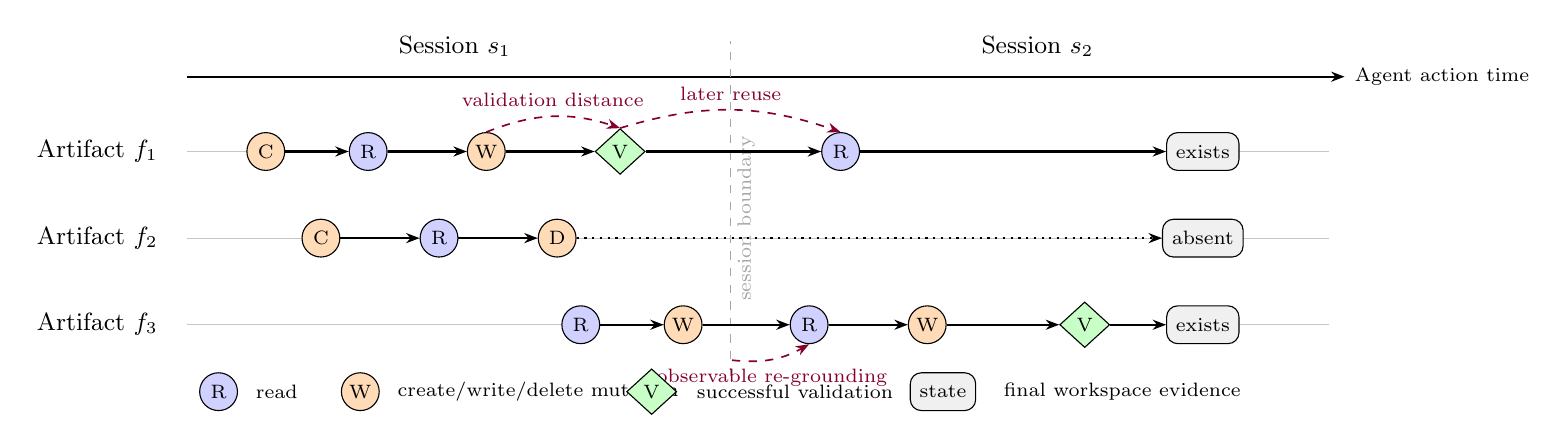
\begin{tikzpicture}[
  x=1cm,y=1cm,
  event/.style={draw,circle,minimum size=0.48cm,font=\scriptsize,inner sep=0pt},
  read/.style={event,fill=blue!18},
  mutate/.style={event,fill=orange!28},
  validate/.style={draw,diamond,aspect=1.5,minimum size=0.58cm,
                   font=\scriptsize,fill=green!22,inner sep=1pt},
  state/.style={draw,rounded corners,minimum height=0.48cm,
                font=\scriptsize,fill=gray!12},
  flow/.style={-{Stealth[length=1.7mm]},thick},
  measure/.style={-{Stealth[length=1.7mm]},dashed,semithick,purple!70!black}
]
\draw[flow] (0.8,3.8) -- (15.5,3.8) node[right,font=\scriptsize] {Agent action time};
\draw[dashed,gray!70] (7.7,0.0) -- (7.7,4.25);
\node[font=\small] at (4.2,4.18) {Session $s_1$};
\node[font=\small] at (11.6,4.18) {Session $s_2$};
\node[font=\scriptsize,rotate=90,gray!70] at (7.9,2.0) {session boundary};

\node[font=\small,anchor=east] at (0.55,2.85) {Artifact $f_1$};
\node[font=\small,anchor=east] at (0.55,1.75) {Artifact $f_2$};
\node[font=\small,anchor=east] at (0.55,0.65) {Artifact $f_3$};
\draw[gray!45] (0.8,2.85) -- (15.3,2.85);
\draw[gray!45] (0.8,1.75) -- (15.3,1.75);
\draw[gray!45] (0.8,0.65) -- (15.3,0.65);

\node[mutate] (c1) at (1.8,2.85) {C};
\node[read] (r1) at (3.1,2.85) {R};
\node[mutate] (w1) at (4.6,2.85) {W};
\node[validate] (v1) at (6.3,2.85) {V};
\node[read] (r2) at (9.1,2.85) {R};
\node[state] (p1) at (13.7,2.85) {exists};
\draw[flow] (c1) -- (r1);
\draw[flow] (r1) -- (w1);
\draw[flow] (w1) -- (v1);
\draw[flow] (v1) -- (r2);
\draw[flow] (r2) -- (p1);

\node[mutate] (c2) at (2.5,1.75) {C};
\node[read] (r3) at (4.0,1.75) {R};
\node[mutate] (d2) at (5.5,1.75) {D};
\node[state] (p2) at (13.7,1.75) {absent};
\draw[flow] (c2) -- (r3);
\draw[flow] (r3) -- (d2);
\draw[flow,dotted] (d2) -- (p2);

\node[read] (r4) at (5.8,0.65) {R};
\node[mutate] (w3) at (7.1,0.65) {W};
\node[read] (rg) at (8.7,0.65) {R};
\node[mutate] (w4) at (10.2,0.65) {W};
\node[validate] (v2) at (12.2,0.65) {V};
\node[state] (p3) at (13.7,0.65) {exists};
\draw[flow] (r4) -- (w3);
\draw[flow] (w3) -- (rg);
\draw[flow] (rg) -- (w4);
\draw[flow] (w4) -- (v2);
\draw[flow] (v2) -- (p3);

\draw[measure] (w1.north) to[bend left=20]
  node[above,font=\scriptsize] {validation distance} (v1.north);
\draw[measure] (v1.north) to[bend left=18]
  node[above,font=\scriptsize] {later reuse} (r2.north);
\draw[measure] (7.72,0.2) to[bend right=18]
  node[below,font=\scriptsize] {observable re-grounding} (rg.south);

\node[read] at (1.2,-0.2) {R};
\node[font=\scriptsize,anchor=west] at (1.55,-0.2) {read};
\node[mutate] at (3.0,-0.2) {W};
\node[font=\scriptsize,anchor=west] at (3.35,-0.2) {create/write/delete mutation};
\node[validate] at (6.7,-0.2) {V};
\node[font=\scriptsize,anchor=west] at (7.15,-0.2) {successful validation};
\node[state] at (10.4,-0.2) {state};
\node[font=\scriptsize,anchor=west] at (11.05,-0.2) {final workspace evidence};
\end{tikzpicture}}
\caption{Measurement schematic for persistent workspace evolution.  Circles
are source-linked reads (R) and mutations (C/W/D); diamonds are successful
validations (V); terminal boxes are independently observed final workspace
state.  Artifact $f_1$ is mutated, validated, reused after a session boundary, and
survives; $f_2$ is created and later deleted; $f_3$ illustrates observable
re-grounding before continued mutation.  The study reports these dimensions
separately and never treats the schematic as empirical data.}
\label{fig:process-measures}
\end{figure*}

\section{Workspace-Centered Measurement}
\label{sec:method}

\subsection{Source Selection and Projection}

We admit a complete native session when its project directory, working
directory or worktree root, or Git remote identifies the target repository.
All Tool actions in an admitted session remain on the timeline, including
searches, shell commands, failed validations, and calls without a resolved
file path.  A global path scan is reported separately because matching only
repository-related lines loses the surrounding no-file actions.

For each admitted action, the projection retains

\begin{equation}
a_i=(t_i,id_i,s_i,v_i,u_i,e_i,q_i),
\end{equation}

where $t_i$ is native time, $id_i$ the stable source ID, $s_i$ the session,
$v_i$ the vendor, $u_i$ the Tool/category, $e_i$ the adapter-derived command
effect, and $q_i$ the reported status.  It attaches zero or more effects

\begin{equation}
\begin{aligned}
E_i &= \{(w,f,o,f')\},\\
o &\in \{\textsf{read},\textsf{write},\textsf{create},\\
  &\qquad \textsf{rename},\textsf{delete}\}.
\end{aligned}
\end{equation}

Here $w$ is a hashed worktree identifier, $f$ is a repository-relative
artifact, and $f'$ is populated only by an observed rename. Failed calls remain
actions but emit no confirmed-success effect.
Directory arguments are weak scope evidence rather than fabricated reads of
every descendant.  Unknown paths, effects, and status remain explicit coverage
gaps.

\begin{figure}[t]
\centering
\resizebox{0.9\columnwidth}{!}{%
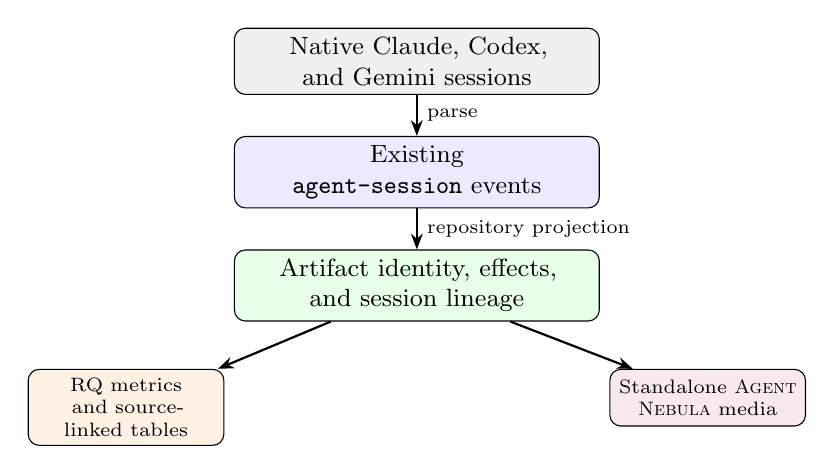
\begin{tikzpicture}[
  box/.style={draw,rounded corners,align=center,minimum height=0.72cm,
              text width=4.4cm,font=\small},
  output/.style={draw,rounded corners,align=center,minimum height=0.72cm,
                 text width=2.25cm,font=\scriptsize},
  flow/.style={-{Stealth[length=2mm]},thick},
  node distance=0.52cm
]
\node[box,fill=gray!12] (native) {Native Claude, Codex, and Gemini sessions};
\node[box,fill=blue!8,below=of native] (parser) {Existing \artifact{agent-session} events};
\node[box,fill=green!9,below=of parser] (projection) {Artifact identity, effects, and session lineage};
\node[output,fill=orange!10,below left=0.6cm and 0.12cm of projection]
  (metrics) {RQ metrics and source-linked tables};
\node[output,fill=purple!9,below right=0.6cm and 0.12cm of projection]
  (media) {Standalone \system media};
\draw[flow] (native) -- node[right,font=\scriptsize] {parse} (parser);
\draw[flow] (parser) -- node[right,font=\scriptsize] {repository projection} (projection);
\draw[flow] (projection) -- (metrics);
\draw[flow] (projection) -- (media);
\end{tikzpicture}}
\caption{One source projection supports measurement and visualization.  The
empirical analyses consume structured events, not visual coordinates.}
\label{fig:architecture}
\end{figure}

\subsection{Artifact and Validation Derivations}

Artifact identity is keyed by hashed worktree ID and relative path. Tool-level
workdir takes precedence over session cwd. An explicit same-worktree rename
preserves identity and its birth state; only a confirmed-success create makes
an identity eligible as an introduction inside the observation. Unknown-status
creates retain a separate birth state. Delete followed by create begins a new identity. For each
confirmed non-delete mutation, we locate later reuse and adapter-recognized
successful validation before the same artifact's next mutation/delete.
Supersession is a competing outcome and only observation end is right-censored.
Final existence and tracked state are queried in the corresponding worktree.

We report complete survival and distance curves or declared sensitivity ranges;
no fixed 24-event attention window enters the research measurement.  Visual
attention decay and force layout remain presentation-only choices.

\subsection{Matched-Comparison Prerequisites}

A valid tool comparison would stratify questions into action-only,
artifact-linked, cross-session, and final-state facts.  Every answer would cite
source IDs or abstain, and no method under comparison could label its own
answer.  Final State and Counts would be lower-information controls, ProcGrep
the strongest action-only procedure baseline, and a bounded raw-log model a
same-source reconstruction condition.

Step 0004 satisfies these prerequisites for the deterministic conditions: it
freezes hashed native prefixes and cutoff state, independently reconstructs
the oracle, and executes the 480-row Final State, Counts, ProcGrep, and
Trajectory matrix.  The Raw branch alone stops during its retrieval-engaged
preflight, so the planned 840-row integrated comparison remains incomplete.
Section~\ref{sec:evaluation} reports the deterministic negative result and
keeps Raw explicitly N/A.

\section{Implementation}
\label{sec:implementation}

The implementation is a Rust extension of the existing \artifact{agentvis}
repository projection.  It reuses \artifact{agent-session} for native parsing,
affiliates sessions with all repository worktrees, normalizes paths, and emits
ordinary source-linked JSON and CSV rows.  The analysis computes project-level
coverage, artifact and mutation rows, and RQ summaries without a frontend,
database, generated semantic layer, or additional runtime dependency.
It reports all admitted Tool actions but uses only actions whose Tool-level
workdir or session cwd resolves to a retained worktree for the primary
activity--progress comparison.

The product path continues to export one standalone HTML, SVG, PNG, GIF, or MP4
per visualization.  Layout is computed once and media outputs share the same
frame stream.  These outputs provide case evidence navigation and reproducible
examples; the empirical measurements are recomputed from structured rows.

\section{Empirical Study}
\label{sec:evaluation}

\subsection{Research Questions}

\paragraph{RQ1---Artifact consolidation and revival.}
How do introduced and repeatedly modified artifacts persist, receive later
reuse, concentrate work, become dormant, and return across Agent action time?

\paragraph{RQ2---Validation response.}
How do successful and failed validations interleave with mutation bursts,
backlog, and subsequent workspace changes?

\paragraph{RQ3---Workspace focus evolution.}
How are path-resolved actions allocated among artifact types, and how do
artifact/module hotspots migrate, cool, and receive later returns?

\paragraph{RQ4---Cross-session continuity.}
What re-grounding and prior-artifact/module continuity is observable between
adjacent non-overlapping native-root session components?

\paragraph{RQ5---Skill and instruction footprints.}
What workspace-action composition is explicitly attributed to named Skills
across independent native root sessions, is it more repeatable than matched
different-Skill activity, and what immediate activity follows explicit
instruction-file access?

\paragraph{RQ6---External boundary.}
Which compatible within-attempt relations replicate in public coding and
scientific-process traces, and which longitudinal claims remain N/A without
persistent cross-session workspace lineage?

\paragraph{Separate tool question---Measurement capability.}
Given the same frozen native evidence and an independent source-explicit
oracle, which action-only, artifact-linked, cross-session, and final-state
facts can Final State, Counts, ProcGrep, bounded raw-log model analysis, and
artifact-linked trajectories answer correctly, and at what evidence and
inference cost?

\subsection{Cases and Inclusion}

We fix six local open-source repositories before computing process rates.
They cover systems software, mixed documentation and code, autonomous research,
and skill/harness development.

\begin{table}[t]
\centering
\small
\begin{tabular}{@{}ll@{}}
\toprule
Repository & Dominant work type \\
\midrule
AgentSight & systems software and research \\
ActPlane & systems software and research \\
bpf-developer-tutorial & tutorial, code, documentation \\
eunomia.dev & content, documentation, software \\
agentskill-observability-paper & paper, experiment, code \\
academic-writing-skills & skills, prompts, tests, documents \\
\bottomrule
\end{tabular}
\caption{Fixed first-study cases.  Each project remains one case; its sessions
are not treated as independent projects.}
\label{tab:cases}
\end{table}

The main corpus includes all repository-direct Claude, Codex, and Gemini
sessions and retains actions with no file effect.  We report source coverage by
project, vendor, session, effect, status, and path presence.  Global path-only
matches form a separate sensitivity analysis.  The corpus contains
551 admitted native root sessions (2,049 source transcript files before
subagent and continuation deduplication) and 181,303 Tool actions; 551 roots
and 176,288 actions resolve to retained worktrees.  It yields 5,746 observed
artifact identities and 13,906 confirmed mutation rows.  All six projects pass
the longitudinal gate, although source coverage for individual measurements
varies substantially.

\subsection{Analysis Protocol}

Each project is first analyzed as a complete case.  Cross-case summaries state
their project weighting and do not treat actions as independent samples.
Primary outputs are effect sizes, distributions, cumulative/survival curves,
and uncertainty.  Bootstrap or permutation uses session or project blocks only
when exchangeability is defensible.  Missing source fields remain coverage
results rather than imputed events.

Artifact type is an inspectable path/extension classification with an unknown
class.  Top-level directories provide the default module unit.  Model-derived
motifs, embeddings, clusters, or summaries are exploratory secondary analyses
and must resolve to source IDs and deterministic metrics.

\subsection{RQ1: Artifact Consolidation and Revival}

RQ1 reports action and mutation volume, introduced-artifact persistence, later
reuse distance, validation-before-supersession distance, competing outcomes,
and the conjunction for eligible observation-born introduction episodes.
Existing-file writes have unknown content durability unless native diffs,
snapshots, or Git line evidence establish it independently.

Figure~\ref{fig:rq1-progress} separates the three dimensions.  All six projects
support later-reuse analysis: 89.3--97.1\% of eligible mutations receive a
later observed access, with delete before reuse treated as a competing outcome.
After projection repair, all six projects also expose an eligible
confirmed create and an adapter-recognized successful validation, so the
preregistered four-project gate admits cross-case interpretation of
persistence and validation (it stopped at 3/6 coverage before repair).  The
six observable persistence proportions are
974/1043, 28/245, 18/30, 8/18, 18/18, and 1/1, and the corresponding observed
validation-before-supersession proportions are 2424/6111, 1212/5604, 141/694,
47/282, 9/196, and 33/247.

\begin{figure*}[t]
  \centering
  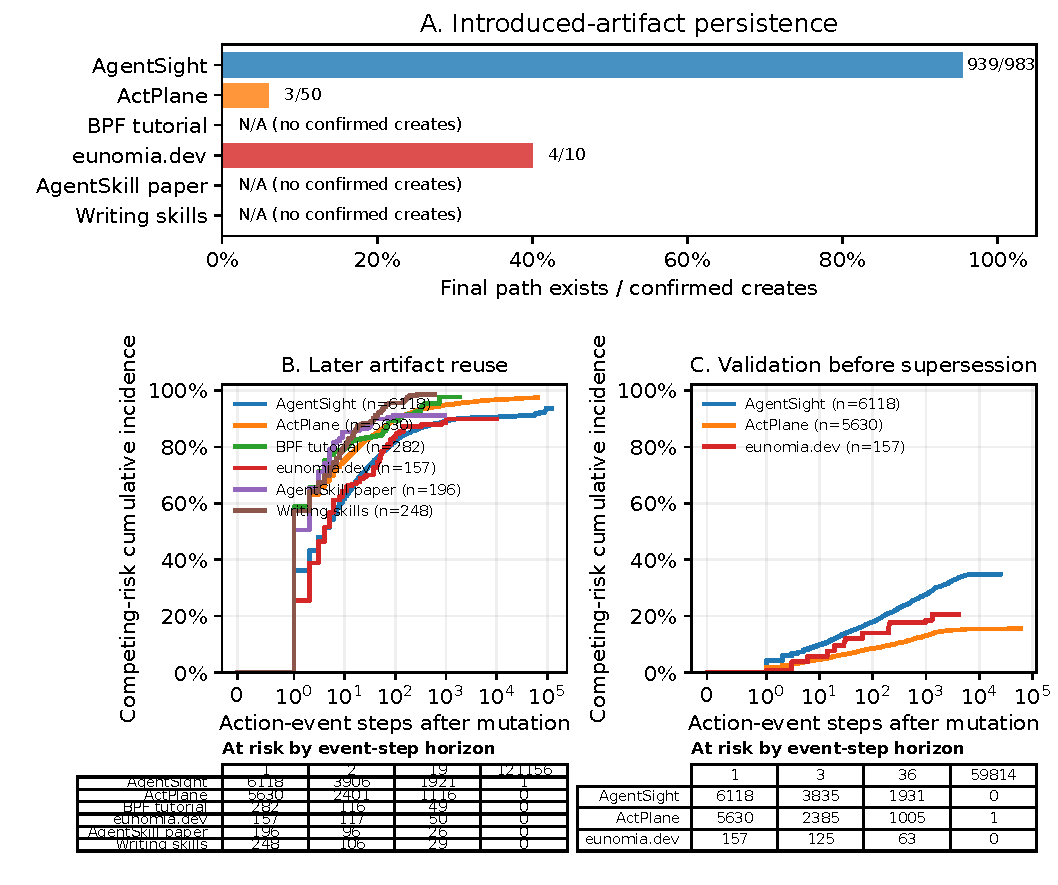
\includegraphics[width=\textwidth]{figures/rq1-progress-curves.pdf}
  \caption{RQ1's three observable progress dimensions.  Panel A reports exact
  final-path persistence only for adapter-recognized confirmed creates.
  Panels B and C use Aalen--Johansen cumulative incidence over native Agent
  action-event distance: deletion competes with later reuse, while the next
  same-artifact mutation/delete competes with recognized validation.  N/A is
  source ineligibility, not zero progress.  After projection repair all 6/6
  cases expose an eligible create and a recognized success (3/6 before
  repair).}
  \label{fig:rq1-progress}
\end{figure*}

Figure~\ref{fig:rq1-activity} tests whether raw action volume is an adequate
proxy for these outcomes.  Reuse covers all six cases, and
its descriptive Spearman rank association with worktree-attributed Tool action
volume is $\rho=0.20$ across six cases.  This weak six-case rank contrast
does not estimate a population effect, but it shows that action count
alone only weakly orders the observed reuse relation in this corpus.  RQ1 thus
establishes measurable activity--progress separation for reuse while, after
repair, also admitting cross-case persistence and validation description.

\begin{figure*}[t]
  \centering
  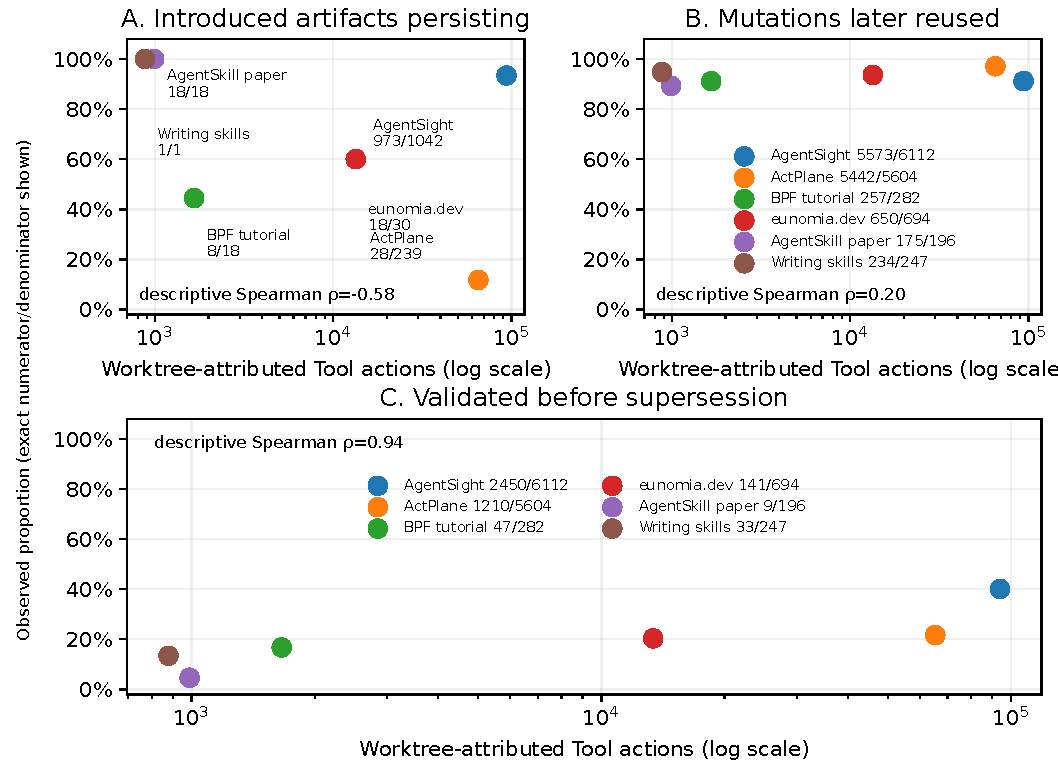
\includegraphics[width=\textwidth]{figures/rq1-activity-progress.pdf}
  \caption{Worktree-attributed Tool action volume versus exact observed RQ1
  proportions.  Labels show numerator/denominator rather than fitted values.
  All three dimensions cover six cases after projection repair; each panel
  reports only a descriptive rank correlation, and actions are not treated as
  independent cases.}
  \label{fig:rq1-activity}
\end{figure*}

\subsection{RQ1 Extension: Dormant-to-Revived Transitions}

We replay confirmed, non-scope artifact touches in native action order,
collapsing compound effects from one action on one identity.  An identity
becomes dormant when consecutive touches are separated by strictly more than
100 intervening Tool actions or strictly more than 24 elapsed hours; its first
subsequent touch is a revival.  This observed lifecycle relation is distinct
from later mutation reuse and is not a progress score.

Table~\ref{tab:rq1-dormancy} reports both thresholds.  Under the action-gap
definition, revived identities account for 8.3--48.3\% of all observed
artifacts and 42.9--75.1\% of artifacts with at least two touches.  The
time-gap definition yields 0.0--40.0\% and 0.0--60.0\%, respectively.  The two
definitions identify 11,271 and 2,285 revival transitions; only 348 and 41
revivals, respectively, are mutations, so revival denotes renewed access
rather than necessarily renewed editing.

\begin{table*}[t]
  \centering
  \footnotesize
  \setlength{\tabcolsep}{3.5pt}
  \begin{tabular}{@{}lrrr rrr@{}}
    \toprule
    & \multicolumn{3}{c}{$>100$ intervening Tool actions}
    & \multicolumn{3}{c}{$>24$ elapsed hours} \\
    \cmidrule(lr){2-4}\cmidrule(l){5-7}
    Project & Revived $n/N$ (\%) & Transitions & Gap med./p90
            & Revived $n/N$ (\%) & Transitions & Gap med./p90 \\
    \midrule
    AgentSight
      & $1{,}271/3{,}267$ (38.9) & 6,856 & 349/4,965.5
      & $526/3{,}267$ (16.1) & 1,086 & 83.1/409.6 \\
    ActPlane
      & $662/1{,}809$ (36.6) & 3,518 & 469.5/5,014
      & $382/1{,}809$ (21.1) & 801 & 81.0/279.2 \\
    bpf-developer-tutorial
      & $42/170$ (24.7) & 73 & 271/661.2
      & $21/170$ (12.4) & 26 & 682.9/3,234.8 \\
    eunomia.dev
      & $174/360$ (48.3) & 805 & 449/2,339
      & $144/360$ (40.0) & 349 & 267.8/1,800.4 \\
    agentskill-observability-paper
      & $2/24$ (8.3) & 3 & 105/120.2
      & $0/24$ (0.0) & 0 & --- \\
    academic-writing-skills
      & $13/116$ (11.2) & 16 & 167.5/360.5
      & $18/116$ (15.5) & 23 & 60.2/605.3 \\
    \bottomrule
  \end{tabular}
  \caption{Per-project dormant-to-revived results under both strict
  thresholds.  Revived identities are reported over all observed identities;
  one identity may contribute multiple transitions.  Gap columns give
  median/p90 intervening Tool actions on the left and elapsed hours on the
  right (Hyndman--Fan type-7 percentiles).}
  \label{tab:rq1-dormancy}
\end{table*}

\subsection{RQ2: Validation Response}

RQ2 measures mutation bursts, recognized successful and failed validation
cadence, and worktree-local mutation accumulation between recognized
successes.  It never calls a successful command proof that every preceding
change was covered or correct.  Figure~\ref{fig:rq2-validation} shows the exact
action-order trajectories and complete inter-success intervals.  After
projection repair, all six projects expose a recognized successful validation
(3/6 before repair), so the predeclared four-project gate admits a cross-case
answer.  Complete intervals are strongly zero-inflated yet
occasionally very large: the seven eligible worktree lanes have 29.3--86.8\%
zero-mutation intervals, while their maxima range from 1 to 817 mutations.
This is evidence about adapter-recognized cadence, not redundant testing or
mutation coverage.

\begin{figure*}[t]
  \centering
  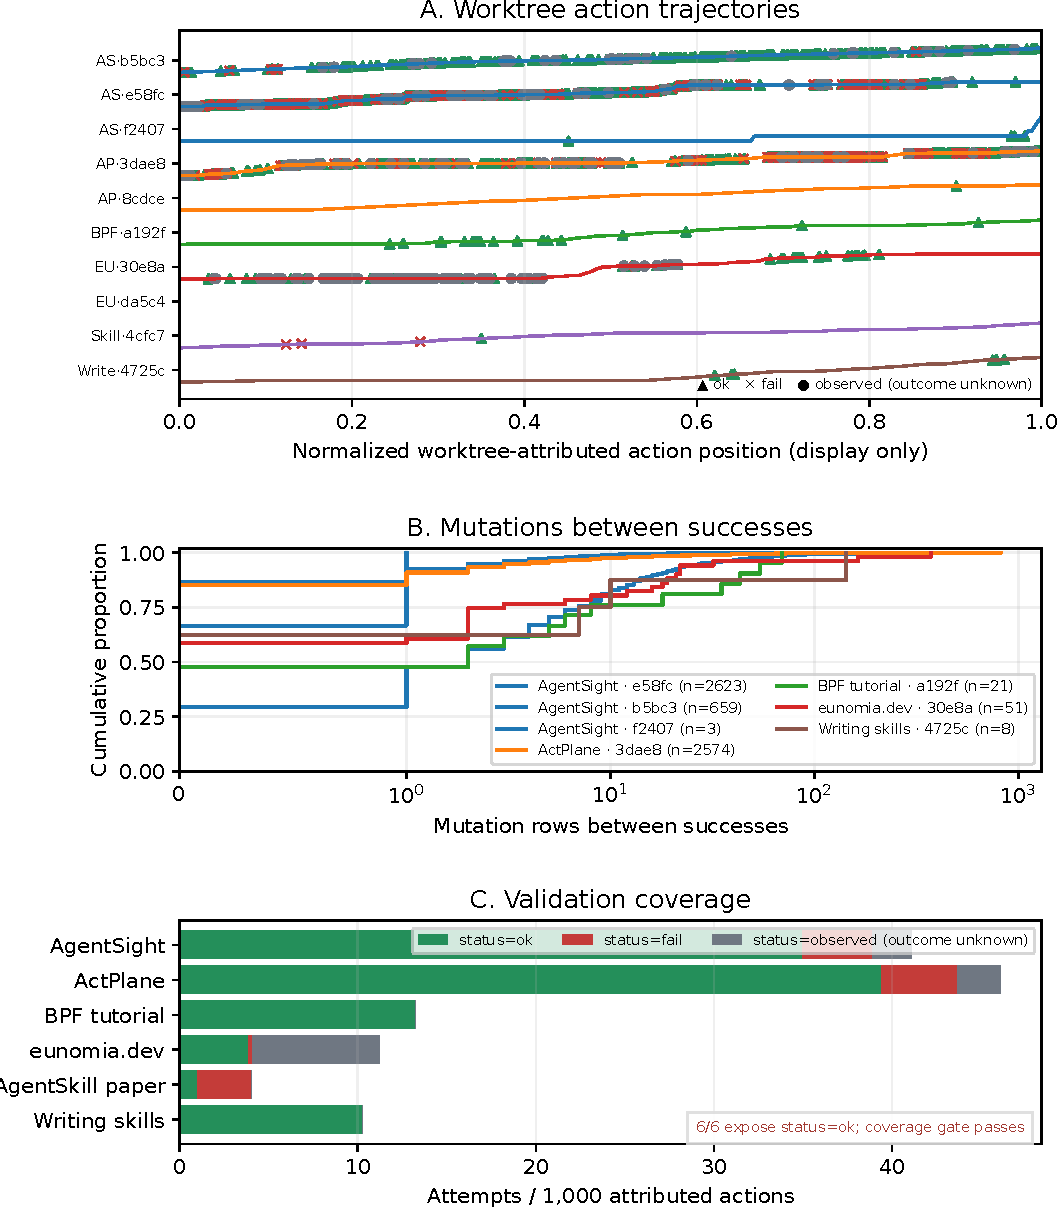
\includegraphics[width=\textwidth]{figures/rq2-validation-dynamics.pdf}
  \caption{RQ2 recognized-validation dynamics.  Panel A follows native Agent
  action order in every worktree lane; mutation effects project to the affected
  worktree while validation remains on the command worktree.  Panel B reports
  complete worktree-local intervals between recognized successful validations.
  Panel C exposes project-level outcome coverage.  All 6/6 cases contain a
  recognized success after projection repair (3/6 before repair).}
  \label{fig:rq2-validation}
\end{figure*}

\subsection{RQ1 Supplement: Repeated-Mutation Structure}

RQ1 also treats each artifact's first observed mutation episode separately from
later observed episodes.  Figure~\ref{fig:rq3-rework} shows that repeat-observed
episodes account for 74.5--90.8\% of observed mutation episodes across all six
qualified cases.  Concentration differs substantially: the exact top 10\% of
mutated identities account for 42.0--86.7\% of episodes.  These are descriptive
properties of the observed trajectories.  They do not identify a tail family,
convergence, thrashing, defect repair, or wasted work; validation-followed
revision and module switching remain open facets of the broader question.

\begin{figure*}[t]
  \centering
  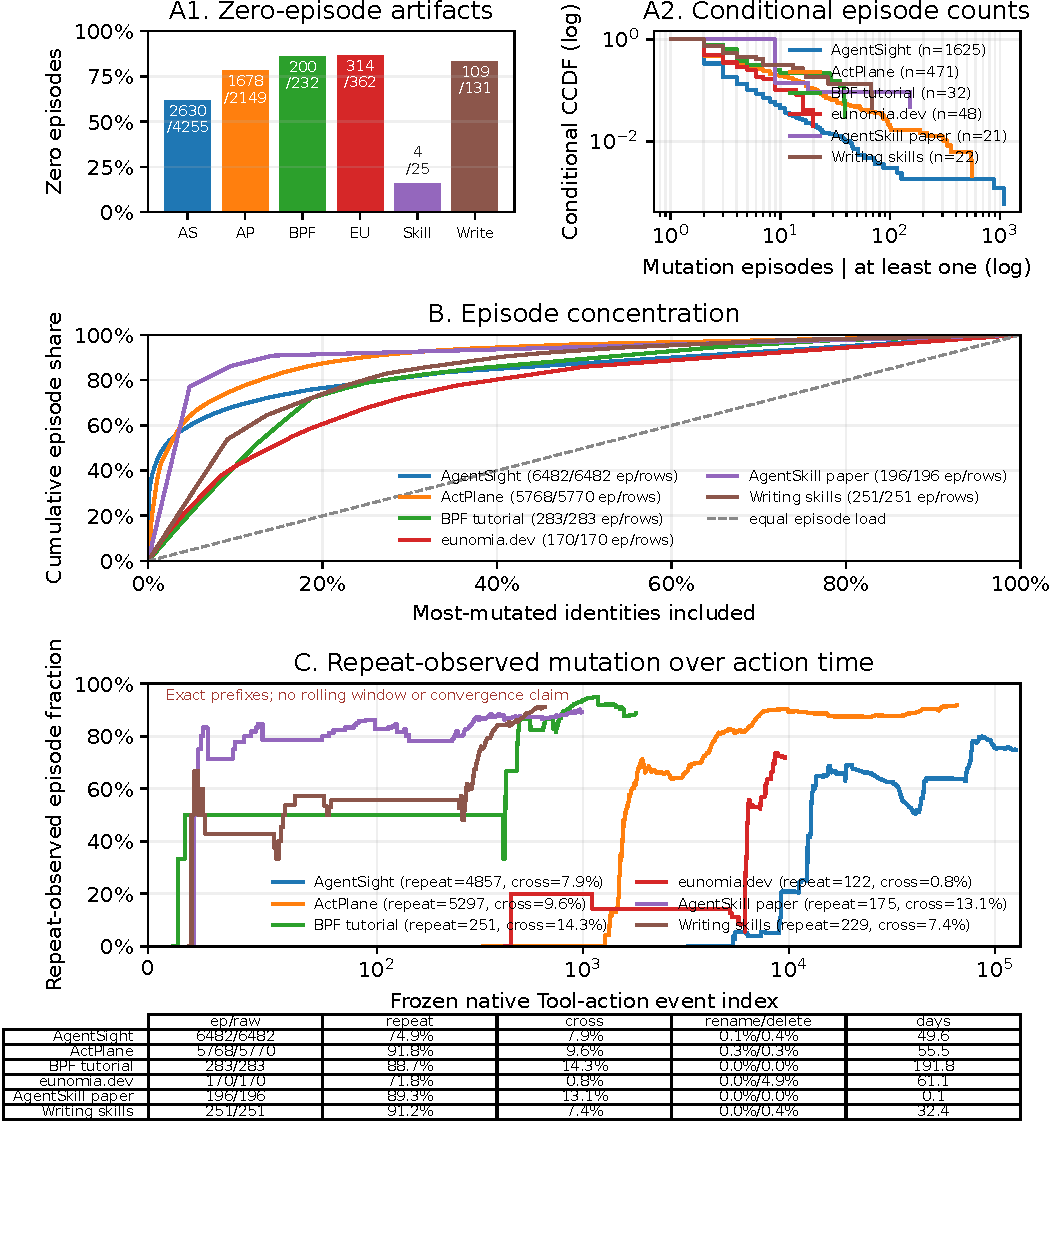
\includegraphics[width=\textwidth]{figures/rq3-rework-structure.pdf}
  \caption{RQ1 repeated-mutation structure for 5,746 observed identities,
  2,431 mutated identities, and 13,860 mutation episodes (13,906 source rows).
  The all-identity zero mass is separated from the conditional CCDF; the
  concentration curve uses the exact fractional 10\% boundary; and the repeat
  fraction evolves as an action-atomic post-action step function.}
  \label{fig:rq3-rework}
\end{figure*}

\subsection{RQ4: Cross-Session Continuity}

Native records expose root/subagent identity unevenly across vendors, and many
source streams share one native root session or overlap in time.  RQ4 therefore
keeps shared-root streams in one independent block and forms transitive concurrency components
within each worktree lane and compares only adjacent non-overlapping
components.  Figure~\ref{fig:rq4-continuity} reports 121 components and 111
boundaries, including mutation-observed prefix composition and defined
artifact/module overlap.  Fewer than four projects reach 20 eligible boundaries
for every estimator; the preregistered gate stops.  A recompute with corrected
native-root and subagent identity confirms the stop is data-limited (three of
six projects reach 20 boundaries), not an artifact of session identity.  The
figure is thus a
source-coverage and within-case continuity audit, not evidence of session reset
cost, resumption, model memory, comprehension, or forgetting.

\begin{figure*}[t]
  \centering
  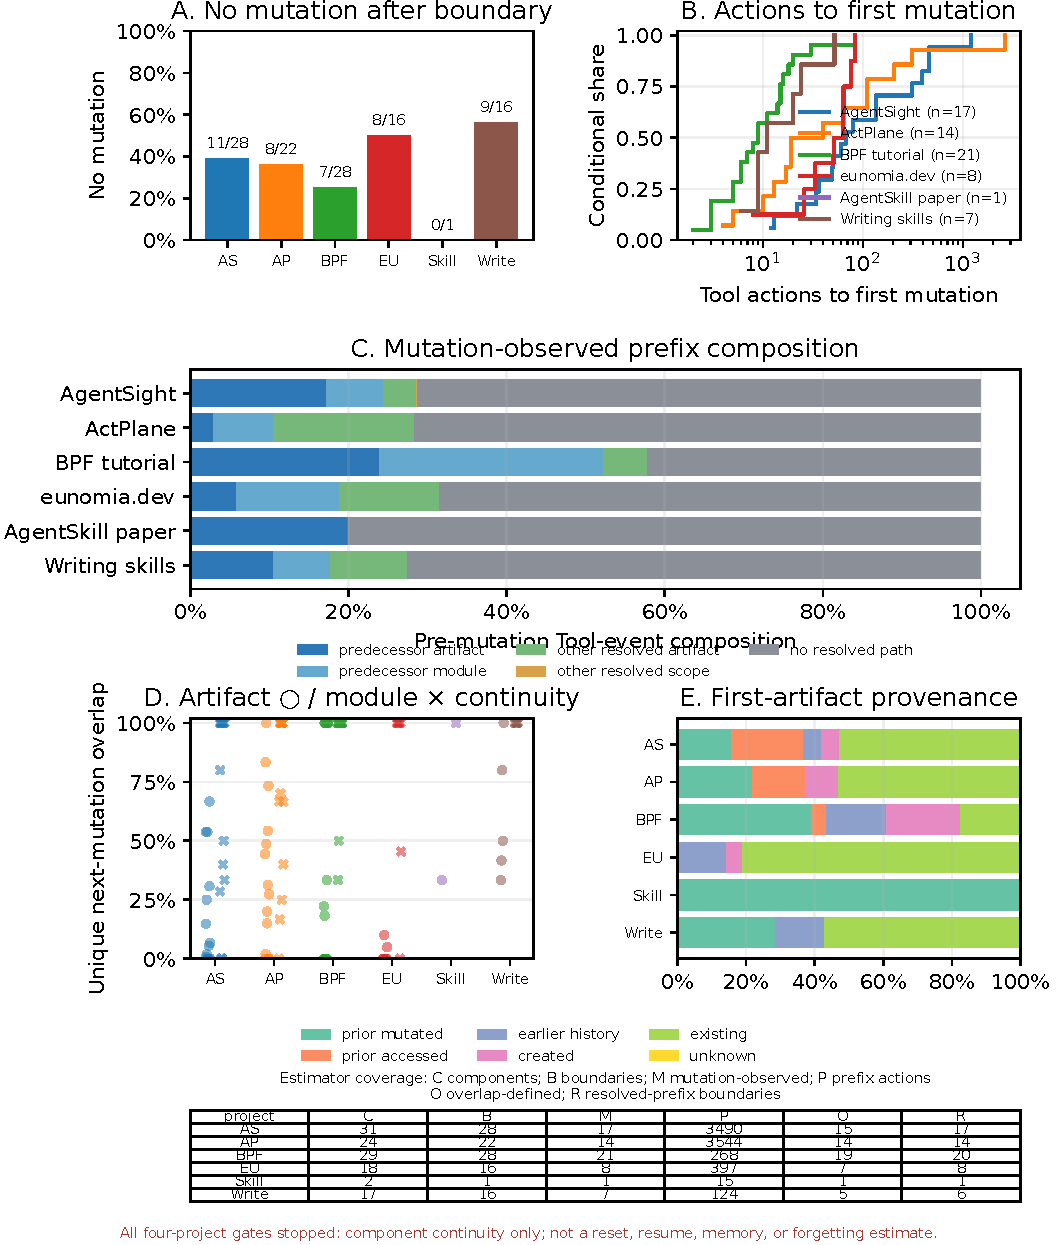
\includegraphics[width=\textwidth]{figures/rq4-component-continuity.pdf}
  \caption{RQ4 source-session component continuity.  Adjacent, non-overlapping
  concurrency components avoid inventing a serial order among overlapping
  sessions.  Timing is conditional on an observed first mutation; empty
  denominators remain undefined.  The stop notice makes the failed
  four-project gate explicit, so all panels remain within-case descriptions.}
  \label{fig:rq4-continuity}
\end{figure*}

\subsection{RQ3: Workspace Focus Evolution}

RQ3 analyzes path-resolved activity rather than latent attention or time spent.
Figure~\ref{fig:rq5-allocation} separates access from mutation and retains both
\texttt{ok} and \texttt{observed} statuses.  Status sensitivity is material:
for example, eunomia.dev's mutation allocation to paper/docs is 39.2\% with all
resolved statuses and 88.2\% with \texttt{ok} only.  Therefore neither stratum
is silently promoted to ground truth.

Figure~\ref{fig:rq5-migration} follows each worktree lane in native call order.
Across the six cases, successive path-resolved calls remain on the same
artifact 29.3--81.6\% of the time, move within the same module 17.5--64.6\%,
and cross modules 0.9--20.8\%.  Five cases meet the return-gap gate, with
median return gaps of 2--4 intervening calls; the AgentSkill case has only three returns
and is N/A.  These path-transition and return measurements do not imply
duration, internal attention, importance, productivity, entropy, or
forgetting; rank-set cooling is analyzed separately below.

\begin{figure*}[t]
  \centering
  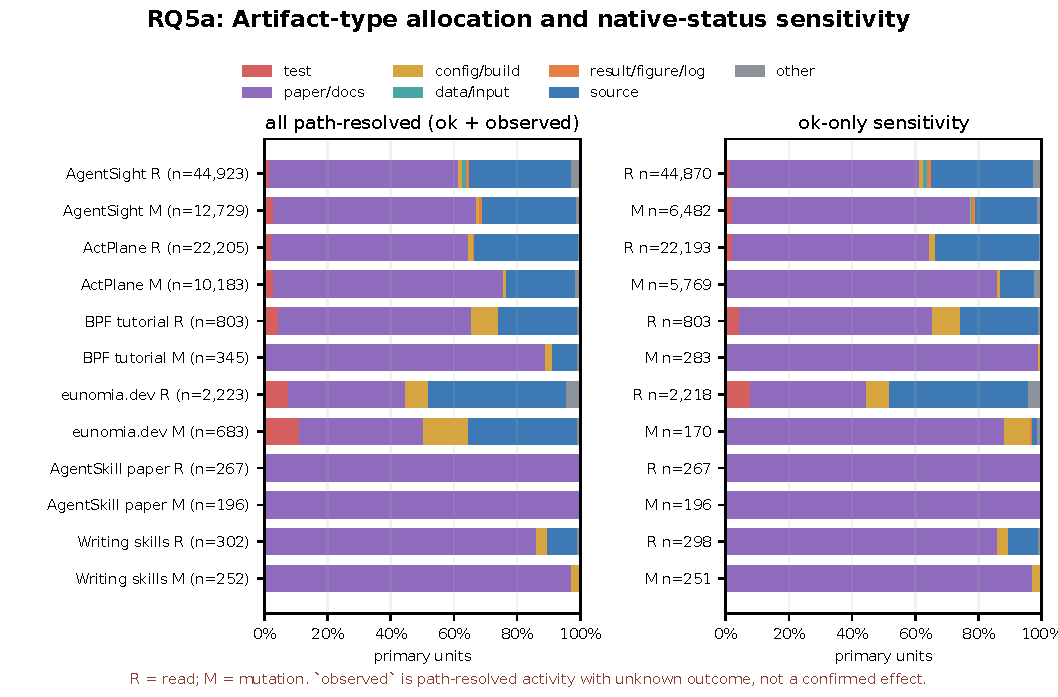
\includegraphics[width=\textwidth]{figures/rq5-artifact-allocation.pdf}
  \caption{RQ3 path-resolved workspace activity allocation by artifact class,
  action effect, and source status.  One multi-path Tool call contributes
  fractionally across its resolved paths in the call-weighted view; exact
  action-weighted rows are retained separately.}
  \label{fig:rq5-allocation}
\end{figure*}

\begin{figure*}[t]
  \centering
  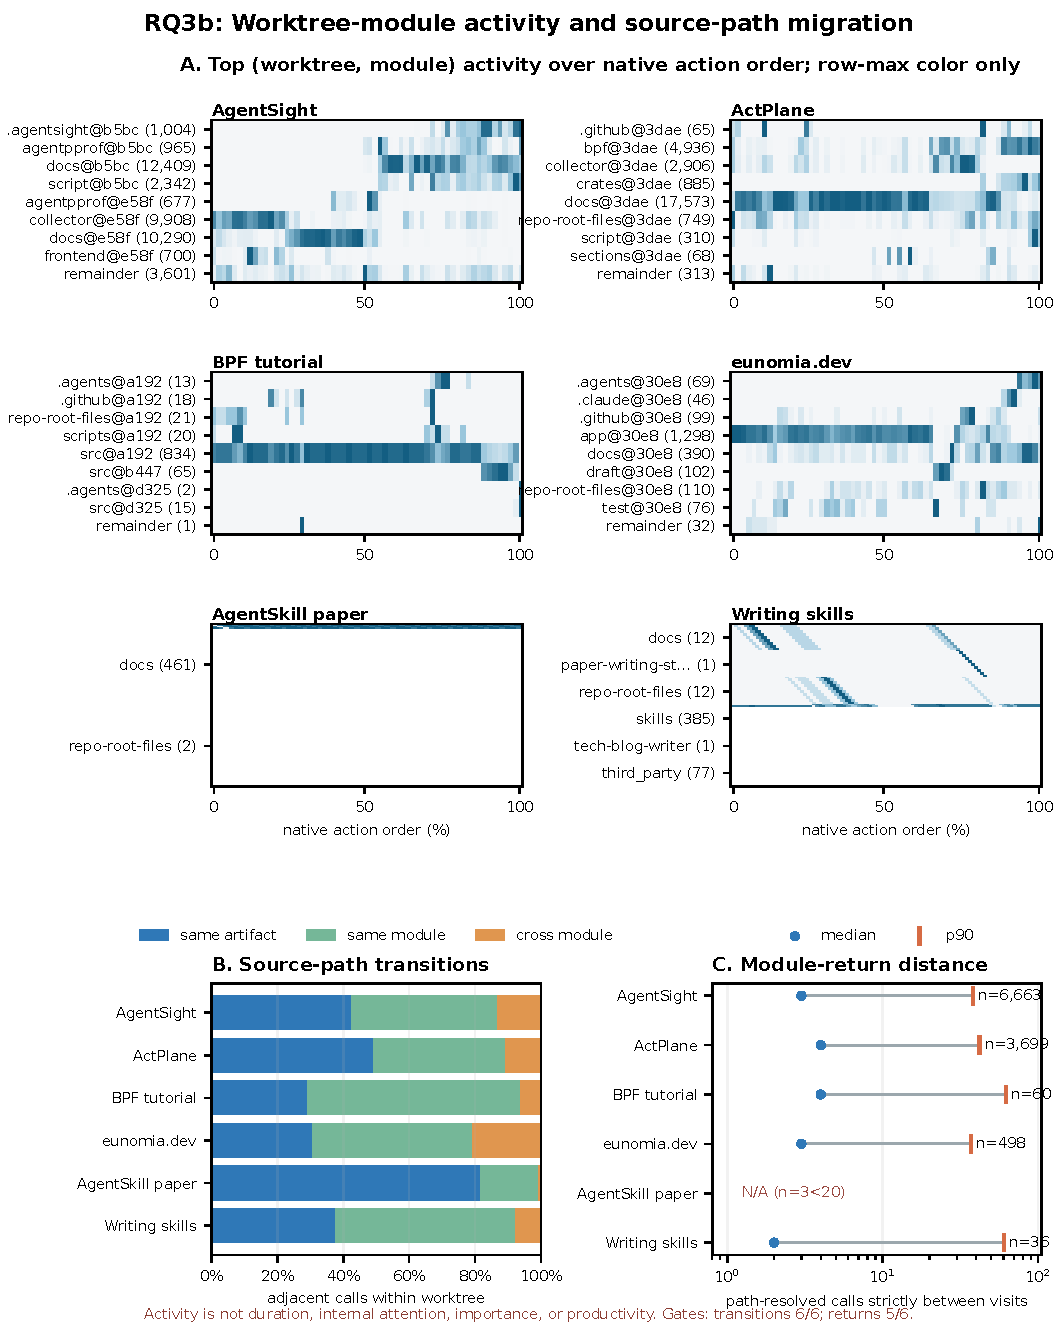
\includegraphics[width=\textwidth,height=0.78\textheight,keepaspectratio]{figures/rq5-activity-migration.pdf}
  \caption{RQ3 workspace focus migration in native call order.  Transitions
  are computed within worktree lanes as same artifact, same module, or cross
  module; return gaps count intervening calls.  Module names and worktree-module
  keys are reported separately, and low-support estimates remain N/A.}
  \label{fig:rq5-migration}
\end{figure*}

\subsection{RQ3 Extension: Rank Turnover and Cooling}

We rank the five most-touched artifacts and top-level modules in 100-action
windows, using a 50-action stride as the primary view and non-overlapping
100-action windows as a sensitivity view.  Across 3,372 nonempty adjacent
primary-window pairs, transition-weighted top-1 changes occur in 49.6\% of
artifact pairs but 13.6\% of module pairs; any top-5 membership change occurs
in 91.5\% versus 42.0\%, and mean membership replacement is 43.5\% versus
17.4\%.  Project medians are similar (50.8\% versus 12.5\%, 88.7\% versus
40.8\%, and 42.9\% versus 20.6\%); the non-overlapping sensitivity preserves
the artifact--module ordering while raising top-1 change to 72.1\% versus
19.1\% and any top-5 change to 97.5\% versus 60.4\%.

For each origin hot-set membership, endpoint retention asks whether the entity
is still hot after a lag, while continuous retention requires membership in
every intervening window.  In the primary view, membership-weighted artifact
endpoint retention falls from 57.0\% at one window to 20.4\% at eight windows,
compared with 84.9\% to 62.7\% for modules; at eight windows, continuous
retention is 4.5\% for artifacts and 41.1\% for modules.  The non-overlapping
eight-window sensitivity gives endpoint retention of 17.1\% versus 58.5\% and
continuous retention of 1.9\% versus 32.1\%.  These are rank-set ``cooling''
curves in Agent action order, not elapsed-time, attention, importance,
productivity, or forgetting measurements.

\subsection{RQ5: Skill and Instruction Footprints}

The corrected parser retains exact \texttt{Skill} names and arguments,
source-native \texttt{attributionSkill}, model, native root-session identity,
source-stream identity, and prompt index.  A separate checker directly rereads
all 2,063 included native transcript streams and reconciles all 7,304 projected
Skill/instruction signal rows and 205,836 adjacent Tool boundaries without a
mismatch.  The six
cases contain 67 explicit Skill invocations and 1,675 source-attributed Skill
Tool actions.

Invocation and execution do not always occupy the same transcript stream: only
476 attributed actions are contiguously preceded by a matching same-stream
invocation.  This is a conservative coverage diagnostic, not an exact join.
We therefore aggregate native-attributed actions by project, vendor, model,
source role, root session, and Skill instead of inventing per-invocation
delegated episode boundaries. Five exact-context Skill strata meet the minimum
of three distinct root sessions, but only
agentskill-observability-paper contains two or more qualified Skills in one
exact project/vendor/model/source-role stratum. Within that case, median
Jensen--Shannon distance is 0.116 for 9 same-Skill pairs and 0.123 for 10
different-Skill pairs.  The median difference is $-0.007$; the one-sided exact
root-block randomization gives $p=0.750$ over 12 admissible assignments (four
distinct statistic values).  The result therefore does not support
a stable or repeatable Skill-fingerprint claim even inside the sole eligible
case.

\begin{figure*}[t]
  \centering
  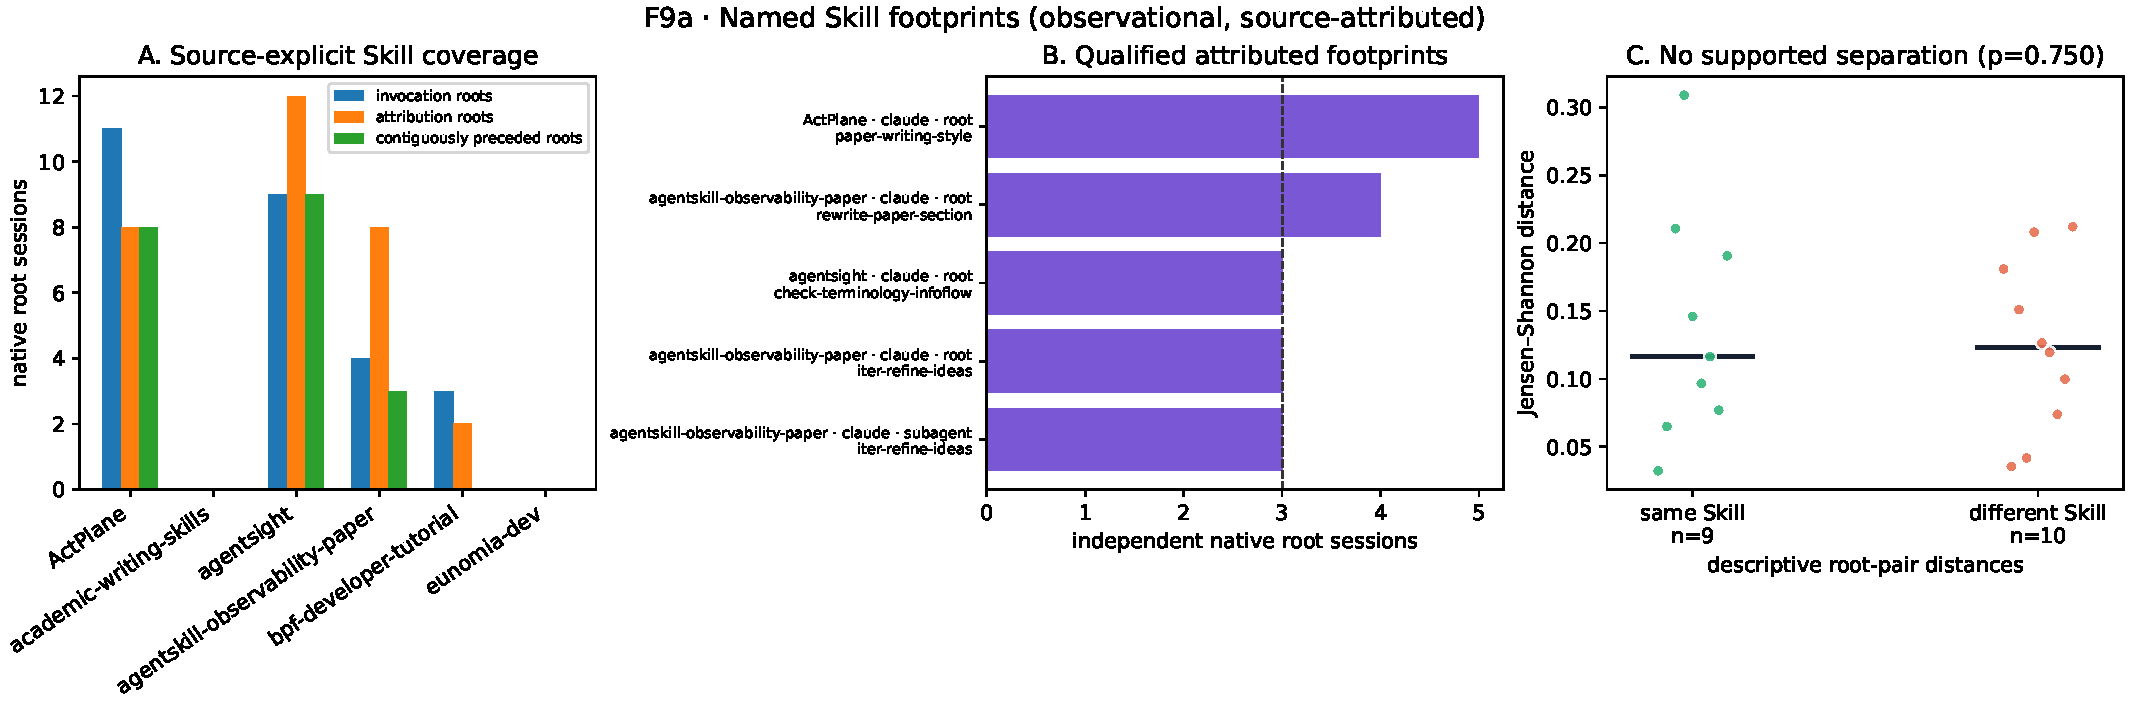
\includegraphics[width=\textwidth]{figures/rq5-skill-footprints.pdf}
  \caption{RQ5 named-Skill evidence.  Transcript files sharing a native root
  session are one independent block.  The support gate requires at least three
  roots.  Same-Skill and different-Skill distances are observational matched
  comparisons, not causal harness effects.}
  \label{fig:rq5-skill-coverage}
\end{figure*}

Reads and mutations of \artifact{AGENTS.md}, \artifact{CLAUDE.md}, and
\artifact{SKILL.md} are analyzed separately as focal events.  Figure
~\ref{fig:rq5-instructions} reports their immediate next Tool action before a
native prompt-index change.  The primary figure uses the 2,822 direct or
simple-shell accesses independently recomputed with high confidence; the
broader parser output remains a sensitivity table because arbitrary scripts
and unexpanded shell globs are not claimed complete.  An access is not proof
that an instruction was injected, followed, useful, or harmful.

\begin{figure*}[t]
  \centering
  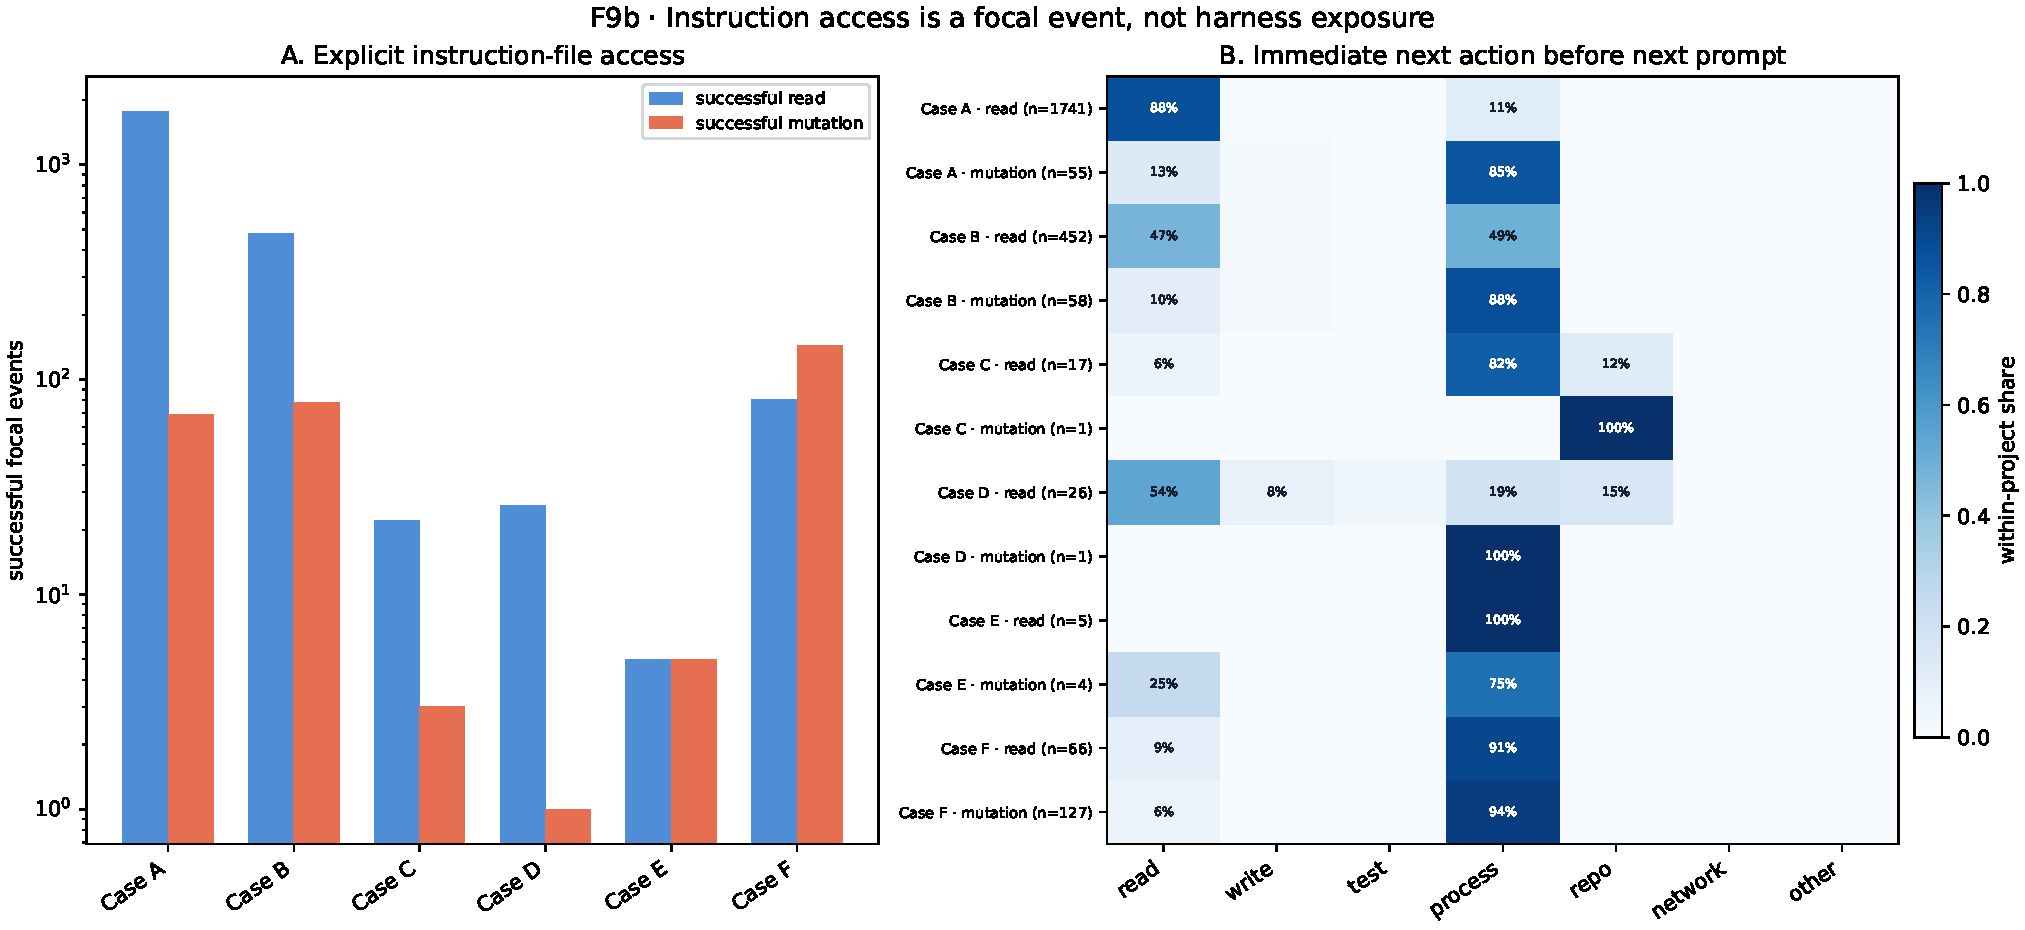
\includegraphics[width=\textwidth]{figures/rq5-instruction-footprints.pdf}
  \caption{RQ5 instruction-file focal events and immediate following activity.
  Reads and mutations remain separate, each focal event contributes at most
  one following Tool action, and next-action shares are normalized within each
  project rather than pooled across the six selected cases.}
  \label{fig:rq5-instructions}
\end{figure*}

\subsection{RQ6: External Boundary}

The six local projects are selected natural cases and do not estimate a
population rate.  We therefore sample 64 independent task instances from each
of four Open-SWE-Traces harness/model strata and 64 independent IdeaTrail
topics (320 stratum-specific selections total; 255 unique Open-SWE task IDs
occur across the 256 Open-SWE selections).  Selection uses a fixed identifier-
hash prefix, and one trajectory is retained per task/topic.  The five
strata are analyzed separately; a second source parser reconciles all 31,249
Tool calls and 22,113 adjacent path-target transitions without a mismatch.

Figure~\ref{fig:rq6-external} reports the exact common estimands.  Aggregate
cross-module movement is 18.0--30.0\% across the public strata, compared with
2.1--20.2\% in the six path-compatible local anchors.  Thus the ordered path
locality relation recurs, but public coding attempts move across top-level
modules more often than most local long-running cases.  Module-return medians
are 2--3 strictly intervening calls publicly and 2--4 in qualified local
cases.  Exploration
before mutation is not a confirmatory result because the public harnesses
shape that order; recognized successful validation lacks a portable
attempt/status pair.  Path concentration and staged revision are analogous
descriptions, not stable-artifact replication.

\begin{figure*}[t]
  \centering
  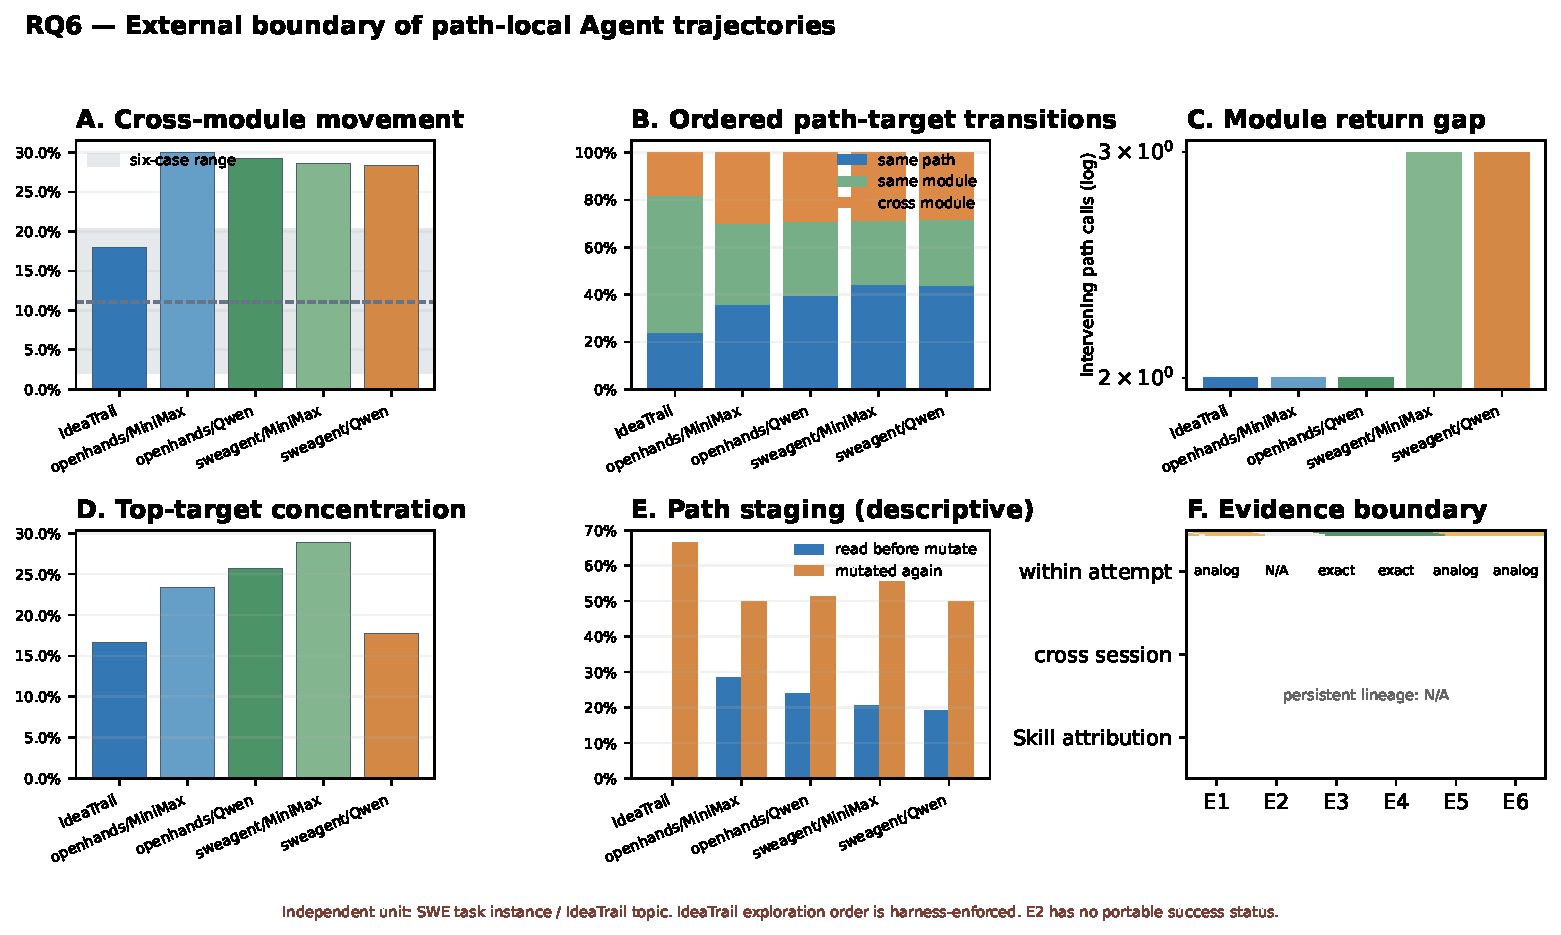
\includegraphics[width=\textwidth]{figures/rq6-external-boundary.pdf}
  \caption{RQ6 external boundary over 64 independent tasks per Open-SWE
  stratum (256 selections, 255 unique task IDs across strata) and 64 IdeaTrail
  topics.  E3/E4 share the local path-target/module-return
  projection; E1/E5/E6 are descriptive or analogous, and E2 is N/A.  Public
  traces do not expose persistent cross-session artifact lineage or exact
  Skill attribution.}
  \label{fig:rq6-external}
\end{figure*}

\subsection{Separate Tool Question: Measurement Capability}

We freeze 12 complete Claude, Codex, or Gemini session files per project and
derive 120 questions: 30 each about action-only, artifact-linked,
cross-session, and final-state facts.  A standalone checker imports neither
the projection code nor \artifact{agent-session}; it reparses the 72 native
files, reconstructs 1,721 artifact edges, independently verifies archived
cutoff state, and reproduces every answer.  We then compare Final State,
Counts, pinned ProcGrep, and the artifact trajectory on the common denominator.

Figure~\ref{fig:rq7-capability} reports the deterministic matrix.  As frozen
on 2026-07-23, Final State answers all 30 final-state questions, and ProcGrep
and Trajectory return identical answers on all 30 action questions while
agreeing with the experiment's different source-direct action grammar on 18.
This does not indicate failed ProcGrep preservation: the official adapter
deliberately leaves some terminal reads unclassified.  The decisive result is
artifact-linked plus cross-session correctness.  The frozen trajectory answers
all 60 questions but returns only 32 correct and 28 wrong, with conditional
accuracy from 0.0 to 1.0 across the six projects.

A follow-up audit classified the 28 errors: 14 were deliberately broader
shell/scope evidence the frozen oracle excludes, and 14 were genuine bugs
(native-root session joins, dropped failed-call effects, shell path
extraction).  Those classes plus one event-workdir bug were repaired, and the
oracle itself was corrected (v4; 24 of 120 expected answers changed, each
justified from source rows).  The current revision answers all 60
artifact-linked and cross-session questions correctly against the corrected
oracle (B 30/30, C 30/30, D 30/30) and 12/30 action-only questions; the
A-family gap is the deliberate grammar difference above, since the trajectory
preserves ProcGrep's action spine while the corrected oracle re-derives atom
counts source-direct.  We report this as repair-corpus conformance on the
six-project benchmark, not as a general exact-fact capability claim.

The bounded Raw-log reader is N/A.  Its single registered Terra preflight made
11 local evidence calls and retrieved 117,184 bytes, but the frozen boundary
monitor stopped execution when an original absolute path embedded in evidence
appeared in a command.  This is a reader-harness contract incompatibility, not
a model result.  We report no Raw accuracy, token, cost, efficiency, or
superiority value.  The deterministic preflight covered all six projects and
is reused as the final deterministic matrix; none of the planned 360 Raw rows
ran.  Deterministic times are also not method-specific because all four methods
share one project-loop measurement.

\begin{figure*}[t]
  \centering
  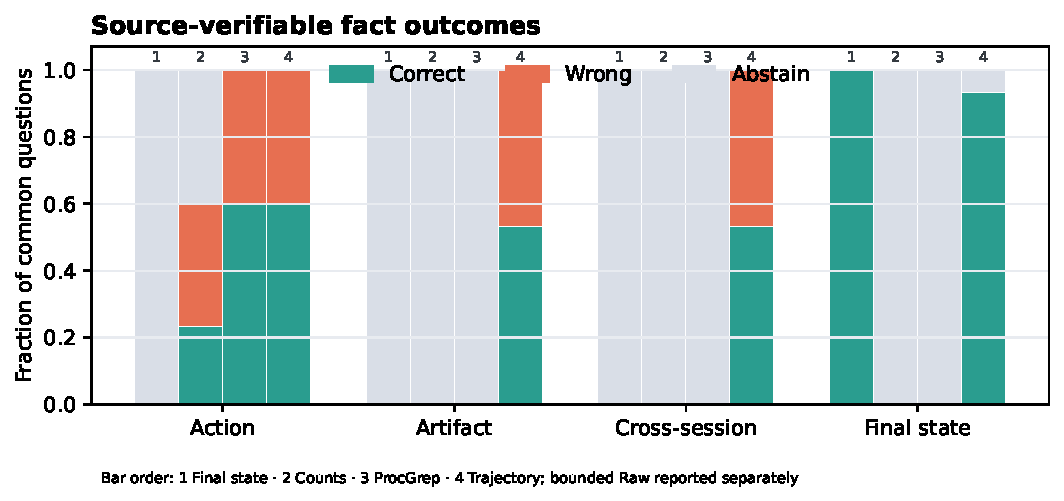
\includegraphics[width=\textwidth]{figures/rq7-measurement-capability.pdf}
  \caption{Source-direct measurement conformance over 120 questions for the
  repaired implementation against the corrected v4 oracle.  Each bar
  partitions the common 30-question family into correct, wrong, and abstain.
  The frozen implementation scored 32/60 on artifact plus cross-session
  families (2026-07-23); after root-cause repair they are 60/60.
  Raw is N/A after its retrieval-engaged preflight stopped at the frozen
  boundary and is not scored as wrong or abstain.}
  \label{fig:rq7-capability}
\end{figure*}

\subsection{Projection Robustness Spot-Checks}

The encoded-Claude-root spot-check covered the one dotted project and all 98 candidate transcript files, found no cwd-less or filter-reliant file and no missing pre-cutoff Tool call, and therefore reports \texttt{corpus\_impact=false}.
The \texttt{plausible\_path\_token} spot-check traced all 652 unique high-confidence rejected event operands to source edges and found zero unmatched operands and zero dropped file-action edges, because this filter gates event path groups rather than the shell-derived file edges.

\section{Threats to Validity}

Native Agent records can omit implicit subprocess effects, external editor
changes, or actions performed outside instrumented tools.  The study reports
adapter and field coverage, and it does not convert missing effects into
no-effect observations.  Optional system-level AgentSight evidence is a future
coverage extension, not a second logic layer in the present analysis.

The source-direct tool experiment also found material disagreement between the
frozen projection and native records: 28/60 answered artifact-linked or
cross-session facts were wrong as of 2026-07-23.  The completed error taxonomy
separated deliberately broader shell/scope admission (14 rows) from genuine
path, artifact-identity, native-root join, and event-workdir errors (14 rows);
the genuine classes were repaired and the oracle corrected.  The current
revision matches the corrected oracle on all 60 B+C questions on this corpus,
and RQ1--RQ4 were recomputed at that revision.  The action-only family still
differs deliberately, because the trajectory preserves ProcGrep's action spine
while the corrected oracle re-derives atom counts source-direct.
RQ5 is better protected by its separate 2,063-stream checker,
and RQ6 by an independent public-data reconstruction.  This repair
removes the frozen conformance objection without turning N/A into observed
absence and without a population-level capability claim.

Final workspace state cannot prove content-level survival of every historical
edit.  We therefore separate file existence, Git-tracked state, and independently
supported content survival.  Successful validation is association rather than
coverage or correctness evidence.

The six cases are selected from local author-associated projects.  They provide
deep, source-native longitudinal evidence but cannot establish population-wide
rates.  The public RQ6 samples independently reproduce only compatible
within-attempt path-locality and return relations.  Open-SWE-Traces consists of
synthetic benchmark attempts, and IdeaTrail is reverse-synthesized under one
workflow; neither validates natural cross-session persistence, re-grounding,
or Skill effects.

Skill, harness, model, task, and project often change together.  Source-native
attribution makes Skill-conditioned activity measurable, but it does not
identify positive and negative configuration exposure or remove task/phase
confounding.  RQ5 therefore reports source-attributed composition and a
negative repeatability result rather than an observational outcome or causal
effect.  Likewise, repeated actions, unvisited artifacts, and long validation
gaps are process facts rather than automatic failure labels.

\section{Related Work}

\paragraph{Agent trajectory studies.}
Software-engineering trajectory studies analyze action sequences, reasoning,
testing, and strategy~\cite{bouzenia2025trajectories,mehtiyev2026behavioral}.
TRAJEVAL identifies coherence collapse after reaching useful intermediate
code~\cite{kim2026trajeval}.  ProcGrep induces canonical action procedures and
behavioral fingerprints~\cite{oderinwale2026procgrep}.  We reuse these
action-level precedents and focus the novelty question on persistent artifact
identity and cross-session lineage.

\paragraph{Long-horizon and persistent work.}
AgingBench studies reliability across many sessions~\cite{zhu2026aging}, while
context-management work shows that plans can lose influence
~\cite{mehta2026plans}.  OR-Space evaluates persistent multi-artifact workspaces
~\cite{zhou2026orspace}.  These works motivate the setting but do not measure
introduced-artifact persistence, reuse, validation association, and re-grounding across
real project histories.

\paragraph{Diagnosis and harness analysis.}
AgentDiagnose and AgentRx diagnose completed trajectories
~\cite{ou2025agentdiagnose,barke2026agentrx}; TrajAudit retrieves evidence from
repository traces~\cite{wang2026trajaudit}; and HarnessFix links failed
trajectories to harness mechanisms~\cite{chen2026harnessfix}.  We do not claim a
new diagnostic labeler or causal harness repair.  Our tool evaluation asks only
which process facts are measurable from source-linked artifact lineage.

\section{Ethical Considerations}

Native trajectories can contain private prompts, source code, paths, secrets,
and experimental data.  Local analysis does not imply permission to publish
raw sessions.  Released evidence must follow repository and data permissions,
remove credentials and personal content, and prefer aggregate or explicitly
approved source-linked examples.

Process measurements can be misused as productivity scores.  We therefore do
not rank people, treat activity volume as progress, or label an observed
pattern as waste without independent task evidence.  The intended consumer is
an Agent or automatic diagnostic process studying its own authorized workspace.

\section{Conclusion}

Long-running Agent work persists in artifacts while session context disappears.
Studying only final state, commits, or action volume therefore misses the
process users need to understand: which work persists, is revisited, receives
recognized validation, accumulates repeated mutation, and migrates across a
workspace.  Across six projects, later reuse is consistently high but weakly
ordered by action volume, while repeated mutation is both common and strongly
concentrated.  Validation, session-continuity, and skill analyses also expose
hard source-coverage boundaries rather than portable success, reset, or causal
harness effects.  Our workspace-centered analysis makes these process facts
inspectable while keeping unsupported comparisons explicitly N/A.  A
source-direct conformance experiment found the frozen projection answering
only 32/60 artifact-linked and cross-session facts correctly (2026-07-23);
root-cause repair brings the current revision to 60/60 against the corrected
benchmark.  The resulting research boundary is concrete---persistent
workspace evolution remains the useful unit, and the repaired projection now
meets source-direct conformance on this corpus while stronger population-level
or tool-capability claims remain out of scope.

\bibliography{references}

\end{document}
